%%%%%%%%%%%%%%%%%%%%%%%%%%%%%%%%%%%%%%%%%%%%%%%%%%%%%%%%%%%%%%%%%%%%%%%%%%%%%%%%%%%%
% Configuración de Paquetes
\documentclass{article}
\usepackage[margin=1in]{geometry} 
\usepackage{amsmath,amsthm,amssymb,amsfonts, fancyhdr, color, comment, graphicx, environ}
\usepackage{xcolor}
\usepackage{mdframed}
\usepackage[shortlabels]{enumitem}
\usepackage{indentfirst}
\usepackage{hyperref}
\usepackage{listings}
\usepackage{karnaugh-map}
\usepackage{booktabs}
\usepackage{geometry}
\hypersetup{
    colorlinks=true,
    linkcolor=blue,
    filecolor=magenta,      
    urlcolor=blue,
}
\setlength{\headheight}{1.5cm}
\renewcommand{\qed}{\quad\qedsymbol}
 % Incluir configuración de paquetes y encabezado
%%%%%%%%%%%%%%%%%%%%%%%%%%%%%%%%%%%%%%%%%%%%%%%%%%%%%%%%%%%%%%%%%%%%%%%%%%%%%%%%%%%%%%%%%%
%Configuración de Enviroments para cuadros de texto
\newenvironment{problem}[2][Ejercicio]
    { \begin{mdframed}[backgroundcolor=gray!20] \textbf{#1 #2} \\}
    {  \end{mdframed}}

\newenvironment{definition}[2][Definición]
    { \begin{mdframed}[backgroundcolor=red!20] \textbf{#1 #2} \\}
    {  \end{mdframed}}

\newenvironment{theorem}[2][Teorema]
    { \begin{mdframed}[backgroundcolor=green!20] \textbf{#1 #2} \\}
    {  \end{mdframed}}

\newenvironment{lemma}[2][Lema]
    { \begin{mdframed}[backgroundcolor=green!20] \textbf{#1 #2} \\}
    {  \end{mdframed}}

\newenvironment{proposition}[2][Proposición]
    { \begin{mdframed}[backgroundcolor=green!20] \textbf{#1 #2} \\}
    {  \end{mdframed}}

\newenvironment{corollary}[2][Corolario]
    { \begin{mdframed}[backgroundcolor=green!20] \textbf{#1 #2} \\}
    {  \end{mdframed}}

\newenvironment{example}[2][Ejemplo]
    { \begin{mdframed}[backgroundcolor=yellow!20] \textbf{#1 #2} \\}
    {  \end{mdframed}}

\newenvironment{remark}[2][Observación]
    { \begin{mdframed}[backgroundcolor=yellow!20] \textbf{#1 #2} \\}
    {  \end{mdframed}}

\newenvironment{note}
    {\textit{Nota:}}
    {}

\newenvironment{conclusion}
    {\textit{Conclusión:}}
    {}

\newenvironment{notation}
    {\textit{Notación:}}
    {}

\newenvironment{question}
    {\textit{Pregunta:}}
    {}

\newenvironment{answer}
    {\textit{Respuesta:}}
    {}
%%%%%%%%%%%%%%%%%%%%%%%%%%%%%%%%%%%%%%%%%%%%%%%%%%%%%%%%%%%%%%%%%%%%%%%%%%%%%%%%%%%%%%%%%% % Incluir configuración de mdframed
%%%%%%%%%%%%%%%%%%%%%%%%%%%%%%%%%%%%%%%%%%%%%%%%%%%%%%%%%%%%%%%%%%%%%%%%%%%%%%%%%%%%

\setlength{\parindent}{0pt}
\pagestyle{fancy}

%Configuraciones adicionales
\binoppenalty=\maxdimen 
\relpenalty=\maxdimen 

%%%%%%%%%%%%%%%%%%%%%%%%%%%%%%%%%%%%%%%%%%%%%
%Condiguracion de encabezado y pie de página
\lhead{Lógica Combinacional}
\rhead{Pedro Villar} 
\chead{}
%%%%%%%%%%%%%%%%%%%%%%%%%%%%%%%%%%%%%%%%%%%%%

\begin{document}

\section*{Sumas de productos y productos de sumas}
Las funciones lógicas se pueden expresar de dos formas diferentes, como una suma de productos o como un producto de sumas. La forma de obtener dicha expresión se basa en identificar que valores de salida tomarán el valor de $1$ y el valor de $0$.
\newline Supongamos que se tiene una función lógica de tres variables $x$, $y$ y $z$, con la siguiente tabla de verdad:

\begin{table}[h]
    \centering
    \begin{tabular}{ccc|c}
        \toprule
        \textbf{x} & \textbf{y} & \textbf{z} & \textbf{S}\\
        \midrule
        0 & 0 & 0 & 0\\
        0 & 0 & 1 & 1\\
        0 & 1 & 0 & 1\\
        0 & 1 & 1 & 0\\
        1 & 0 & 0 & 1\\
        1 & 0 & 1 & 0\\
        1 & 1 & 0 & 0\\
        1 & 1 & 1 & 1\\
        \bottomrule
    \end{tabular}
\end{table}

\begin{enumerate}
    \item Para expresar como \textbf{suma de productos}, se toman los minitérminos que hacen que la función devuelva $1$, luego se suman los minitérminos.
    \item Para expresar como \textbf{producto de sumas}, se toman los maxitérminos que hacen que la función devuelva $0$, luego se multiplican los maxitérminos.
\end{enumerate}

\begin{table}[h]
    \centering
    \begin{tabular}{cccccc}
        \toprule
        \textbf{x} & \textbf{y} & \textbf{z} & \textbf{S} & \textbf{Minterminos} & \textbf{Maxiterminos}\\
        \midrule
        0 & 0 & 0 & 0 & $m_0 = x'y'z'$ & $M_0 = x+y+z$\\
        0 & 0 & 1 & 1 & $m_1 = x'y'z$ & $M_1 = x+y+z'$\\
        0 & 1 & 0 & 1 & $m_2 = x'yz'$ & $M_2 = x+y'+z$\\
        0 & 1 & 1 & 0 & $m_3 = x'yz$ & $M_3 = x+y'+z'$\\
        1 & 0 & 0 & 1 & $m_4 = xy'z'$ & $M_4 = x'+y+z$\\
        1 & 0 & 1 & 0 & $m_5 = xy'z$ & $M_5 = x'+y+z'$\\
        1 & 1 & 0 & 0 & $m_6 = xyz'$ & $M_6 = x'+y'+z$\\
        1 & 1 & 1 & 1 & $m_7 = xyz$ & $M_7 = x'+y'+z'$\\
        \bottomrule
    \end{tabular}
\end{table}

Con esto se tienen las formas canónicas de la función lógica, las cuales se pueden simplificar utilizando mapas de Karnaugh.
\begin{itemize}
    \item \textbf{Suma de productos:} $S = m_1 + m_2 + m_4 + m_7 = x'y'z + x'yz' + xy'z' + xyz$,
    \item \textbf{Producto de sumas:} $S = M_0 \cdot M_3 \cdot M_5 \cdot M_6 = (x+y+z)(x+y'+z')(x'+y+z')(x'+y'+z)$.
\end{itemize}


\newpage

\section*{Mapas de Karnaugh}

\begin{mdframed}[backgroundcolor=red!40,shadow=true,shadowsize=2pt,roundcorner=2pt]
    Los mapas de Karnaugh son una herramienta útil que nos permite aplicar un método de simplificación de funciones lógicas.
\end{mdframed}

El Mapa de Karnaugh tiene la característica de que puede ser visto como una representación bidimensional de una tabla de verdad. En la tabla de verdad, se colocan las variables por columnas y las combinaciones de tales variables determinan un valor de salida, 0 o 1, sin embargo, en el mapa las variables se colocan como si de un plano cartesiano se tratara, respetando cada una de las combinaciones que de ellas se generan, y colocando en la intersección de las combinaciones de las variables, el valor de salida.

\begin{figure}[h]
    \centering
    \begin{karnaugh-map}[4][4][1][$w$][$z$][$y$][$x$]
        \minterms{0,1,2,3,4,8,9,11,12}
        \autoterms[0]
        \implicant{0}{8}{red}
        \implicant{0}{2}{blue}
        \implicant{0}{1}{green}
    \end{karnaugh-map}
    \caption{Ejemplo de un mapa de Karnaugh}
\end{figure}

Los mapas muestran la relación que existe entre  las entradas y las salidas de un circuito lógico, si se aplica adecuadamente el resultado será el más simplificado posible. Pueden ser utilizados para cualquier número de variables de entrada sin embargo se recomienda un máximo de seis variables.

\subsection*{Representación de tabla de verdad en un mapa de Karnaugh}
Las tablas de la verdad se pueden representar en un mapa de Karnaugh, para ello se deben seguir los siguientes pasos:
\begin{enumerate}
    \item Se deben identificar los términos de la tabla de verdad que son 1.
    \item Se deben identificar los términos de la tabla de verdad que son 0.
    \item Se deben identificar los términos de la tabla de verdad que son 1 y que se pueden agrupar.
    \item Se deben identificar los términos de la tabla de verdad que son 0 y que se pueden agrupar.
\end{enumerate}

\begin{mdframed}[backgroundcolor=blue!40,shadow=true,shadowsize=2pt,roundcorner=2pt]
    Observaciones:
    \begin{itemize}
        \item Los términos de la tabla de verdad que son 1 se representan en el mapa de Karnaugh con un $1$, y sirven para expresar a la función como una suma de productos.
        \item Los términos de la tabla de verdad que son 0 se representan en el mapa de Karnaugh con un $0$ y sirven para expresar a la función como un producto de sumas.
    \end{itemize}
\end{mdframed}
\newpage

\subsection*{Ejemplo de representación de tabla de verdad en un mapa de Karnaugh}
Supongamos que se tiene la siguiente tabla de la verdad:

\begin{table}[h]
    \centering
    \begin{tabular}{ccccc}
        \toprule
        \textbf{x} & \textbf{y} & \textbf{z} & \textbf{w} & \textbf{S}\\
        \midrule
        0 & 0 & 0 & 0 & 0\\
        0 & 0 & 0 & 1 & 1\\
        0 & 0 & 1 & 0 & 1\\
        0 & 0 & 1 & 1 & 0\\
        0 & 1 & 0 & 0 & 1\\
        0 & 1 & 0 & 1 & 0\\
        0 & 1 & 1 & 0 & 0\\
        0 & 1 & 1 & 1 & 1\\
        1 & 0 & 0 & 0 & 1\\
        1 & 0 & 0 & 1 & 0\\
        1 & 0 & 1 & 0 & 0\\
        1 & 0 & 1 & 1 & 1\\
        1 & 1 & 0 & 0 & 0\\
        1 & 1 & 0 & 1 & 1\\
        1 & 1 & 1 & 0 & 1\\
        1 & 1 & 1 & 1 & 0\\
        \bottomrule
    \end{tabular}
\end{table}
Para hacer un mapa de Karnaugh, primero se separan las variabes $xy$ y $zw$ y se colocan en el mapa de la siguiente forma:

\begin{figure}[h]
    \centering
    \begin{karnaugh-map}[4][4][1][$w$][$z$][$y$][$x$]
        %\minterms{3,4,5,6,7,9,12,13,14}
        \autoterms[-]
    \end{karnaugh-map}
    \caption{Mapa de Karnaugh para las variables $xy$}
\end{figure}

\newpage
Luego identificamos los términos de la tabla de verdad que son 1 y los colocamos en el mapa de Karnaugh.
\newline Por ejemplo esta linea de la tabla
\begin{table}[h]
    \centering
    \begin{tabular}{ccccc}
        \toprule
        \textbf{x} & \textbf{y} & \textbf{z} & \textbf{w} & \textbf{S}\\
        \midrule
        0 & 0 & 0 & 1 & 1\\
        \bottomrule
    \end{tabular}
\end{table}

Se coloca en el mapa de Karnaugh en la posición donde $xy$ toma $00$ y $zw$ toma $01$.

\begin{figure}[h]
    \centering
    \begin{karnaugh-map}[4][4][1][$w$][$z$][$y$][$x$]
        \minterms{1}
        \autoterms[0]
        \implicant{1}{1}{red}
    \end{karnaugh-map}
    \caption{Ejemplo de representación}
\end{figure}

Pasar por cada linea de la tabla de verdad y colocar los términos en el mapa de Karnaugh. Los términos que no son $1$ se colocan como $0$ en el mapa de Karnaugh.

\begin{figure}[h]
    \centering
    \begin{karnaugh-map}[4][4][1][$x$][$y$][$z$][$w$]
        \minterms{1,2,4,7,8,11,13,14}
        \autoterms[0]
    \end{karnaugh-map}
    \caption{Mapa de Karnaugh completo del ejemplo.}
\end{figure}

\newpage
\subsection*{Agrupación de términos}
Para simplificar la función lógica, se deben agrupar los términos que son 1 en el mapa de Karnaugh. Los términos se pueden agrupar siguiendo las siguientes reglas:

\begin{enumerate}
    \item Los grupos deben contener una cantidad de elementos igual a potencias de 2. Es decir, los grupos solo podrán realizarse con cantidades de celdas iguales a: 1, 2, 4, 8, 16, 32, etc.
    \item Se deben generar grupos con combinaciones de variables adyacentes, es decir, sólo debe de haber un cambio entre cada una de las combinaciones, por ejemplo la combinación $ABC'$ es adyacente con $AB'C'$ , ya que sólo cambia la variable $B$.
    \item Grupos en las posiciones en los extremos y esquinas del mapa. Las posiciones de los extremos y las esquinas son adyacentes, por lo que se pueden agrupar. Esta adyacencia se debe a que el mapa de Karnaught puede ser visto como un toroide.
    \item Grupos de unos darán lugar a una suma de productos o mini términos.
    \item Grupos de ceros darán lugar a un producto de sumas o maxi términos.
    \item Los grupos deben ser lo más grande posible. Se buscará realizar grupos con la mayor cantidad de elementos posibles, entre más grande el grupo, se obtiene una función más simplificada. 
    \item No se pueden generar grupos en diagonal. Solo se permitirán grupos en vertical y horizontal dentro del mapa.
    \item Puede existir solapamiento de grupos, siempre y cuando exista al menos un elemento que no haya sido agrupado anteriormente.
    \item No deben existir grupos redundantes, es decir, no se puede realizar un grupo dentro de otro grupo, y no se puede realizar un grupo con elementos que ya hayan sido completamente agrupados en otros conjuntos.
\end{enumerate}

Por ejemplo, si se tiene este mapa de Karnaugh:

\begin{figure}[h]
    \centering
    \begin{karnaugh-map}[4][4][1][$x$][$y$][$z$][$w$]
        \minterms{4,12,6,14,0,2}
        \autoterms[0]
    \end{karnaugh-map}
    \caption{Mapa de Karnaugh para agrupar.}
\end{figure}

\newpage
Se debería agrupar de la siguiente forma:

\begin{figure}[h]
    \centering
    \begin{karnaugh-map}[4][4][1][$w$][$z$][$y$][$x$]
        \minterms{4,12,6,14,0,2}
        \autoterms[0]
        \implicantedge{0}{4}{2}{6}{green}
        \implicantedge{4}{12}{6}{14}{red}
    \end{karnaugh-map}
    \caption{Mapa de Karnaugh agrupado.}
    \label{fig:karnaugh_agrupado}
\end{figure}

\subsection*{Simplificación de la función lógica}
Para la simplificación de la función lógica, se usan los grupos que se han formado en el mapa de Karnaugh. Cada grupo se convierte en un término de la función lógica, y se deben sumar los términos que se obtienen de los grupos, teniendo en cuenta lo siguiente:

\begin{enumerate}
    \item Si un grupo es de una sola celda, se incluye igualmente en la función lógica.
    \item En el grupo, las variables que cambian de valor "se me van" del término, y las que no cambian su valor permanecen.
    \item Si un grupo se solapa con otro, no cambia la forma de trabajarlos, cada grupo es un término distinto.
\end{enumerate}

Por ejemplo, tomando el mapa de Karnaugh anterior, se obtiene la siguiente función lógica:
\begin{equation*}
    F = x'w' + yw'
\end{equation*}

\newpage
\subsection*{Resumen}

\subsubsection*{Simplificación de términos}
\begin{mdframed}[backgroundcolor=yellow!40,shadow=true,shadowsize=2pt,roundcorner=2pt]
    \begin{enumerate}
        \item Se agrupan ya sean $1$'s o $0$'s, en potencias de 2.
        \item Se pueden agrupar en vertical, horizontal o en todas las esquinas. Una forma de verlo es como un pacman, siempre las celdas por donde podría moverse son agrupables.
        \item Para armar los términos, se mantienen las variables que no cambian de valor y se eliminan las que cambian.
        \item Luego se suman o multiplican los términos obtenidos, dependiendo si se quiere expresar como suma de productos o producto de sumas.
    \end{enumerate}
\end{mdframed}

\subsubsection*{Método para expresar como suma de productos simplificada}
\begin{mdframed}[backgroundcolor=yellow!40,shadow=true,shadowsize=2pt,roundcorner=2pt]
    \begin{enumerate}
        \item Dibujar la tabla y luego el mapa de Karnaugh de la dimensión correcta, asignar nombre y valor a las filas y columnas.
        \item Llenar los $1$'s y $0$'s donde correspondan (Véase la Figura \ref{fig:karnaugh_agrupado} de ejemplo.)
        \item Agrupar los $1$'s adyacentes en cuadrados o rectangulos lo mas grande posible.
        \item Todos los $1$'s quedan agrupados si o sí, si no se pueden juntar con otros queda el grupo de una sola celda.
        \item Representar cada término como un producto (dejando las variables que no cambian de valor) y sumarlos.
        \item El resultado es la función expresada como \textbf{suma de productos}.
    \end{enumerate}
\end{mdframed}

\subsubsection*{Método para expresar como producto de sumas simplificada}
\begin{mdframed}[backgroundcolor=yellow!40,shadow=true,shadowsize=2pt,roundcorner=2pt]
    \begin{enumerate}
        \item Dibujar la tabla y luego el mapa de Karnaugh de la dimensión correcta, asignar nombre y valor a las filas y columnas.
        \item Llenar los $1$'s y $0$'s donde correspondan.
        \item Agrupar los $0$'s adyacentes en cuadrados o rectangulos lo mas grande posible, considerando que la cantidad de celdas debe ser potencia de 2.
        \item Cada grupo de $0$'s se convierte en un término de la función lógica simplificada.
        \item Representar cada término como una suma (dejando las variables que no cambian de valor) y multiplicarlos.
    \end{enumerate}
\end{mdframed}

\newpage
\section*{PLA: Programmable Logic Array}
Programmable Logic Array (PLA) es un dispositivo lógico de arquitectura fija con puertas AND programables seguidas de puertas OR programables. PLA es básicamente un tipo de dispositivo lógico programable que se utiliza para construir un circuito digital reconfigurable. La estructura de un PLA es la siguiente:

\begin{figure}[h]
    \centering
    \includegraphics[scale=0.2]{PLA.png}
    \caption{Estructura de un PLA}
\end{figure}

El funcionamiento se podria resumir en tres pasos:

\begin{enumerate}
    \item \textbf{Programación:} el usuario define la función lógica que se desea implementar.
    \item \textbf{Generación de términos del producto:} las entradas se aplican a la matriz de puertas AND para producir un conjunto de términos de producto.
    \item \textbf{Generación de suma de términos:} los términos de producto se aplican a la matriz de puertas OR para producir la salida.
\end{enumerate}

\subsection*{Método para implementar una función lógica en un PLA}
\begin{mdframed}[backgroundcolor=red!40,shadow=true,shadowsize=2pt,roundcorner=2pt]
    \begin{enumerate}
        \item Una vez se tenga la función lógica simplificada, se deben identificar los términos de la función.
        \item Cada término de la función se convierte en una fila de la matriz de puertas AND.
        \item Luego se suman los términos de la función y se convierten en una fila de la matriz de puertas OR.
        \item La salida de la matriz de puertas OR es la función lógica implementada en el PLA.
    \end{enumerate}
\end{mdframed}

\newpage
\section*{Ejemplo completo de Lógica Combinacional}
Un detector de paridad impar de 4 entradas y una salida funciona de la siguiente manera: si la cantidad de entradas con valor ‘1’ es impar la salida se pone en ‘1’, en el resto de los casos la salida toma valor ‘0’
\begin{enumerate}[a)]
    \item Construir la tabla de verdad para dicho sistema.
    \item Obtener la ecuación lógica como suma de minitérminos y producto de maxitérminos (funciones canónicas).
    \item Implementar el sistema con compuertas NAND de la cantidad de entradas requeridas.
    \item Implementar el sistema con una PLA.
\end{enumerate}

\subsection*{Punto a}
Para construir la tabla de verdad, se deben considerar las 4 entradas posibles y la salida que se obtiene para cada combinación de entradas.

\begin{table}[h]
    \centering
    \begin{tabular}{cccc|c|c|c}
        \toprule
        \textbf{A} & \textbf{B} & \textbf{C} & \textbf{D} & \textbf{S} & \textbf{Minitérminos} & \textbf{Maxitérminos}\\
        \midrule
        0 & 0 & 0 & 0 & 0 & $m_0$ = A'B'C'D' & $M_0$ = A+B+C+D\\
        0 & 0 & 0 & 1 & 1 & $m_1$ = A'B'C'D & $M_1$ = A+B+C+D'\\
        0 & 0 & 1 & 0 & 1 & $m_2$ = A'B'CD' & $M_2$ = A+B+C'+D\\
        0 & 0 & 1 & 1 & 0 & $m_3$ = A'B'CD & $M_3$ = A+B+C'+D'\\
        0 & 1 & 0 & 0 & 1 & $m_4$ = A'BC'D' & $M_4$ = A+B'+C+D\\
        0 & 1 & 0 & 1 & 0 & $m_5$ = A'BC'D & $M_5$ = A+B'+C+D'\\
        0 & 1 & 1 & 0 & 0 & $m_6$ = A'BCD' & $M_6$ = A+B'+C'+D\\
        0 & 1 & 1 & 1 & 1 & $m_7$ = A'BCD & $M_7$ = A+B'+C'+D'\\
        1 & 0 & 0 & 0 & 1 & $m_8$ = AB'C'D' & $M_8$ = A'+B+C+D\\
        1 & 0 & 0 & 1 & 0 & $m_9$ = AB'C'D & $M_9$ = A'+B+C+D'\\
        1 & 0 & 1 & 0 & 0 & $m_{10}$ = AB'CD' & $M_{10}$ = A'+B+C'+D\\
        1 & 0 & 1 & 1 & 1 & $m_{11}$ = AB'CD & $M_{11}$ = A'+B+C'+D'\\
        1 & 1 & 0 & 0 & 0 & $m_{12}$ = ABC'D' & $M_{12}$ = A'+B'+C+D\\
        1 & 1 & 0 & 1 & 1 & $m_{13}$ = ABC'D & $M_{13}$ = A'+B'+C+D'\\
        1 & 1 & 1 & 0 & 1 & $m_{14}$ = ABCD' & $M_{14}$ = A'+B'+C'+D\\
        1 & 1 & 1 & 1 & 0 & $m_{15}$ = ABCD & $M_{15}$ = A'+B'+C'+D'\\
        \bottomrule
    \end{tabular}
\end{table}

\subsection*{Punto b}
Para obtener la ecuación lógica como suma de minitérminos y producto de maxitérminos, se deben identificar los términos que hacen que la función devuelva $1$ y los términos que hacen que la función devuelva $0$.

\begin{itemize}
    \item \textbf{Suma de minitérminos:} tomo los términos que hacen 1 la función y los sumo.
    \begin{equation*}
        F = m_1 + m_2 + m_4 + m_7 + m_8 + m_{11} + m_{13} + m_{14}
    \end{equation*}
    Desarrollando la ecuación, se obtiene:
    \begin{equation*}
        F = A'B'C'D + A'B'CD' + A'BC'D' + A'BCD + AB'C'D' + AB'CD + ABC'D + ABCD'
    \end{equation*}

    \item \textbf{Producto de maxitérminos:} tomo los términos que hacen 0 la función y los multiplico.
    \begin{equation*}
        F = M_0 \cdot M_3 \cdot M_5 \cdot M_6 \cdot M_9 \cdot M_{10} \cdot M_{12} \cdot M_{15}
    \end{equation*}
    Desarrollando la ecuación, se obtiene:
    \begin{align*}
        F &= (A+B+C+D)(A+B+C'+D')(A+B'+C+D')(A+B'+C'+D)(A'+B+C+D') \\
        & (A'+B+C'+D')(A'+B'+C+D)(A'+B'+C'+D')
    \end{align*}
\end{itemize}

\newpage
\subsection*{Punto c}
Para implementar el sistema con compuertas NAND, se deben seguir los siguientes pasos:
\begin{enumerate}
    \item Se toma la forma canónica de la función lógica, en este caso se tomará la forma de suma de minitérminos.
    \item Luego se niega dos veces la función lógica, para obtener la forma de producto de maxitérminos.
    \item Se aplica una vez más la ley de De Morgan para obtener la forma buscada.
\end{enumerate}

\begin{align*}
    F &= A'B'C'D + A'B'CD' + A'BC'D' + A'BCD + AB'C'D' + AB'CD + ABC'D + ABCD' \\
    &= (A'B'C'D + A'B'CD' + A'BC'D' + A'BCD + AB'C'D' + AB'CD + ABC'D + ABCD')'' \\
    &= (A'B'C'D)' \cdot (A'B'CD')' \cdot (A'BC'D')' \cdot (A'BCD)' \cdot (AB'C'D')' \cdot (AB'CD)' \cdot (ABC'D)' \cdot (ABCD')'
\end{align*}

\subsection*{Punto d}
Para implementar el sistema con una PLA, se utilizará la forma canónica de la función lógica, en este caso se tomará la forma de suma de minitérminos.

\begin{figure}[h]
    \centering
    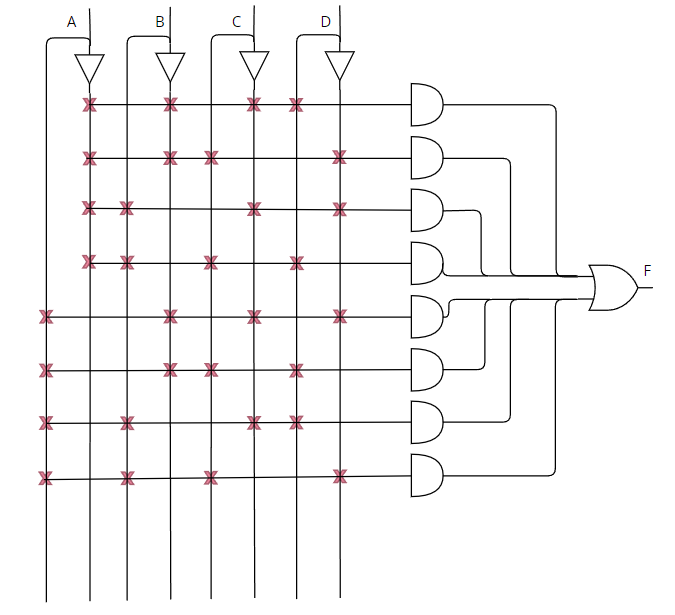
\includegraphics[scale=0.8]{plaej.png}
    \caption{Estructura de la función lógica en una PLA.}
\end{figure}

\end{document}